% !TEX TS-program = pdflatex
% !TEX encoding = UTF-8 Unicode

% This is a simple template for a LaTeX document using the "article" class.
% See "book", "report", "letter" for other types of document.

\documentclass[11pt]{article} % use larger type; default would be 10pt

\usepackage[utf8]{inputenc} % set input encoding (not needed with XeLaTeX)
\usepackage{float}
\usepackage{mathtools}
\usepackage{microtype}

%%% Examples of Article customizations
% These packages are optional, depending whether you want the features they provide.
% See the LaTeX Companion or other references for full information.

%%% PAGE DIMENSIONS
\usepackage{geometry} % to change the page dimensions
\geometry{a4paper} % or letterpaper (US) or a5paper or.... 
%\geometry{margin=1in} % for example, change the margins to 2 inches all round
% \geometry{landscape} % set up the page for landscape
%   read geometry.pdf for detailed page layout information

\usepackage{graphicx} % support the \includegraphics command and options

% \usepackage[parfill]{parskip} % Activate to begin paragraphs with an empty line rather than an indent

%%% PACKAGES
\usepackage{booktabs} % for much better looking tables
\usepackage{array} % for better arrays (eg matrices) in maths
\usepackage{paralist} % very flexible & customisable lists (eg. enumerate/itemize, etc.)
\usepackage{verbatim} % adds environment for commenting out blocks of text & for better v\usepackage{subfigure} % make it possible to include more than one captioned figure/table in a single float
% These packages are all incorporated in the memoir class to one degree or another...
\usepackage{subfigure}
\usepackage{caption}
%\usepackage{subcaption}

%\DeclareCaptionFormat{subfig}{\figurename~#1#2#3}
%\DeclareCaptionSubType*{figure}
\captionsetup[subfigure]{format=subfig,labelsep=colon,labelformat=simple}


%%% HEADERS & FOOTERS
\usepackage{fancyhdr} % This should be set AFTER setting up the page geometry
\pagestyle{fancy} % options: empty , plain , fancy
\renewcommand{\headrulewidth}{0pt} % customise the layout...
\lhead{}\chead{}\rhead{}
\lfoot{}\cfoot{\thepage}\rfoot{}

%%% SECTION TITLE APPEARANCE
\usepackage{sectsty}
%\allsectionsfont{\sffamily\mdseries\upshape} % (See the fntguide.pdf for font help) % (This matches ConTeXt defaults)
%%% ToC (table of contents) APPEARANCE
%\usepackage[nottoc,notlof,notlot]{tocbibind} % Put the bibliography in the ToC
\usepackage[titles,subfigure]{tocloft} % Alter the style of the Table of Contents
\renewcommand{\cftsecfont}{\rmfamily\mdseries\upshape}
\renewcommand{\cftsecpagefont}{\rmfamily\mdseries\upshape} % No bold!


\usepackage{listings}
\usepackage{color}
\usepackage{microtype}
\usepackage{hyperref} % use hyperlinked ToC
\hypersetup{colorlinks=true, linkcolor=black}

\definecolor{dkgreen}{rgb}{0,0.6,0}
\definecolor{gray}{rgb}{0.5,0.5,0.5}
\definecolor{mauve}{rgb}{0.6,0,0.6}

\lstset{frame=tb,
  %language=C++,
  aboveskip=3mm,
  belowskip=3mm,
  showstringspaces=false,
  columns=flexible,
  basicstyle={\small\ttfamily},
  numbers=left,
  numberstyle=\tiny\color{gray},
  keywordstyle=\color{mauve},
  commentstyle=\color{dkgreen},
  stringstyle=\color{mauve},
  breaklines=true,
  breakatwhitespace=true
  tabsize=3
}
%%% END Article customizations
%%% The "real" document content comes below...
\title{RTDSP Project: Speech Enhancement}
\author{Joshua Elsdon je310, Oskar Weigl ow610}
%\date{} % Activate to display a given date or no date (if empty),
         % otherwise the current date is printed 

\begin{document}
\maketitle
\center{\textbf{\large{\emph{"...a profound trust in the advances of science."}	}}}

\abstract{
Noise reduction from audio is of great importance, especially when applied to telecommunications.
What this project aims to do is demonstrate some of the techniques that are available to reduce the noise from a multitude of sources.
We use a number of techniques in series, such as background subtraction and a non-linear method based on SRN thresholding, producing excellent results; reducing the noise drastically in all situations.
\tableofcontents
\clearpage


\section{Introduction} 
In this project we aim to produce a real-time filtering algorithm that will remove a variety noise sources from a sample recording. The filtering operation needs to be effective on all noise sources without sample-specific modifications.
The basic form for all these filters will be to find the background noise signature then to subtract that from the recording, which is known as \emph{Spectral Subtraction}. 

\section{Simple Implementation of Spectral Subtraction} 
\label{sec:simple}
In this implementation we track the noise floor in the sample by finding the minimum amplitude of each bin of an FFT. We continually update this estimate during a 2.5s period, after which we save it into an array for future reference, and start on a new 2.5 second period.
We hold 4 samples of the estimated noise floor amplitude, one from each of the aforementioned periods. This includes the current estimate.
To estimate the overall noise floor, we select from each bin the minimum amplitude from each of the saved periods.
We then subtract the amplitude of the noise floor spectrum from the amplitude of the input spectrum. This then becomes the de-noised output of our initial implementation.
In order to continue the process, at each 2.5 second period we shift the noise floor examples in our buffers, deleting the last one to maintain exactly 4 samples of the noise floor amplitude. The code that achieves this can be seen in Appendix~\ref{app:simple}. It uses pointers to arrays to do efficient rotations of all bins simultaneously.

The implementation has two tuning parameters, \verb"alpha" and \verb"lambda". \verb"alpha" controls the amplification factor that is applied to the model noise floor before subtraction: very low values give insufficient noise attenuation, very high values start to distort the speech making it sound somewhat like the speaker is underwater. A value of between 2 and 10 makes for the most audible speech, varying depending on the source of noise present. 
\verb"lambda" is the value setting the minimum value that the noise floor is allowed to take, as on a occasion the noise floor could be considered negative (and hence we would actually add more noise upon subtraction). This should be kept low, in fact we found that a value of 0 works the best. In this case, it ensures that the noise floor cannot be considered negative, and all positive values will pass through unchanged.


\section{Low pass filtering $\lvert X(\omega) \rvert $} 
\label{sec:LPF}
\begin{figure}[htbp]
	\begin{center}
    \begin{lstlisting}[language = C]
for (k = 0; k < FFTLEN; ++k) {
	float curramp = cabs(procframe[k]); 

	curramp = (1-kop1)*curramp + kop1*ampbinstate[k];
	ampbinstate[k] = curramp;

	float currnoisebin = clearM ? curramp : min(Mbuffs[0][k], curramp);
	Mbuffs[0][k] = currnoisebin;

	for (i = 1; i < NumMbuff; ++i)
		currnoisebin = min(currnoisebin, Mbuffs[i][k]);

	currnoisebin *= alpha;

	float g = max(lambda, 1-(currnoisebin/curramp));
	procframe[k] = rmul(g, procframe[k]);
}
    \end{lstlisting}
  \end{center}
	\caption{Code segment showing the implementation of low pass filtering the FFT of the input. kop1 is the scaling factor that places the pole of the low pass filter.}
	\label{code:LPFxOMG}
\end{figure}

This enhancement tries to combat the inaccuracies of taking the minimum value of each bin to represent the noise floor. This problem manifests because often the minimum for each bin is not representative of the actual noise floor, hence the need for large alpha values times. By using a low pass filter, single low values in a particular bin are given less influence on the current noise floor model, and they will need to remain low for a number of frames to suggest that that particular bin is indeed required to be lower to be representative of the noise floor.
This filtering is applied directly to the FFT of the input and therefore we can use the same minimum search method of finding the noise floor of each bin. The low pass filtering code segment is shown in Figure~\ref{code:LPFxOMG}. Line number \verb"4" performs the IIR filter. 

The effect of this enhancement is very noticeable, the words are less corrupted by the subtraction of the noise, due the fact that our estimation of the noise is much more representative of the actual noise floor.   
\section{Filtering Using Spectral Power} 
\subsection{Low pass filtering $\lvert X(\omega) \rvert^{2} $} 

This enhancement is very similar to that presented in Section~\ref{sec:LPF} though instead of using the amplitude, then IIR filtering it, we IIR filter the power spectrum instead, this is a benefit as it makes a larger difference between quieter background noise, and the louder signal we are trying to extract. This should enhance our ability to extract the noise floor. 

In reality this enhancement added little to the sound quality of the output, bordering on inaudible changes. Though the method of filtering in the power domain will be used to great effect later in the string of enhancements.  

\subsection{Generating $g(\omega)$ Using Ratios of Power} 
\label{sec:powerrat}
\begin{equation}
\label{equ:powerRat}
	g(\omega) = \max\left(\lambda, \sqrt{1- \frac{\lvert N(\omega) \rvert ^{2}}{\lvert X(\omega) \rvert ^{2}}}\right)
\end{equation}

This enhancement generates $g(\omega)$ using the ratio of signal and noise power rather than of amplitude(Equation~\ref{equ:powerRat}), where $g(\omega)$ is the current filter multiplier that is to be applied to the input. Using power ratios instead of amplitude ratios has makes the $g(\omega)$ emphasise sounds with larger amplitude much more than those with small amplitude, as the low pass filtering will be linear with power instead of with amplitude. If we assume that the signal amplitude is always significantly more than that of the noise, then this helps the selectivity of the filter quite significantly.

This aided the performance of our system, though once again the affect was marginal. The strange sounds that were present in the low frequencies (especially in the car sample) where somewhat reduced, though the actual clarity of the speech was not affected greatly.

\subsection{Generating $g(\omega)$ Using Ratios of Low pass filtered power} 
\label{sec:powerratLPF}
\begin{equation}
\label{equ:powerRatLPF}
	g(\omega) = \max\left(\lambda, \sqrt{1- \frac{\lvert N(\omega) \rvert ^{2}}{\lvert P(\omega) \rvert ^{2}}}\right)
\end{equation}

We attempted to use the equation listed in Equation~\ref{equ:powerRatLPF}. This is the same as in Section~\ref{sec:powerrat} but using the low pass filtered version of the input spectrum to generate the power spectrum. This was quite successful at removing musical noise in the factory sample, though introduced significant reverberation. The musical noise was able to be suppressed as the filter will only open after the SNR has been good for some time. As such it acts as a SNR sensitive compressor.
The reverberations that appear are due the filter ($g(\omega)$) changing directly as a result of the current data, which causes nonlinear feed-forward in the system. That is, as a attack from the voice comes, the initial attack makes it through the filter from the first sample. Then, as the filter opens with the time-constant of $P(\omega)$, a second artificial attack is perceived. We try to remedy this problem in Section~\ref{sec:delayprepipe}.

\subsection{Low Pass Filtered Power With Look-ahead}
\label{sec:delayprepipe}

We added a single stage buffer for the input, such that the data that is now old by one frame period is shaped by the information contained in the newest frame period. This was in an attempt to break the feed-forward that was causing reverberation in Section~\ref{sec:powerratLPF}.
As the filter shape now depends on the next frame rather than the current frame, the feed-forward should be less sharp. The success of this implementation was limited, there was slightly reduced reverberation, but the overall improvement was not significant. The code for this section is listed in Appendix~\ref{app:delayprepipe}. This particular modification was rolled back and not used for the final code.

\section{Zeroing Bins That Fall Bellow Threshold SNR} 

In this enhancement we wished to remove the small chirping noises that are left over in from the previous enhancements. Generally the chirping is much quieter that the speech after the techniques discussed previously, so we implemented a simple routine that drives the bins, which have insufficient estimated SNR, to zero.

This has the effect of making the sections with no speech completely silent, so long as there is no musical noise. This is because after previous filtering, all bins fall below our threshold and can be removed completely. Musical noise still gets through this filter in general as it has not been suppressed sufficiently from the previous stages of enhancement. Furthermore, noise that is still present in the speech itself, despite the subtraction, is dwarfed by the speech signal itself. Thus the fact that this SNR thresholding does nothing to help this part of the noise, is of no concern.

A further improvement to this enhancement was to weigh the SNR cutoff threshold by the smoothed estimated total noise power over all frequencies. This is so that  when there is a large amount of noise the nonlinear zeroing will be less aggressive.
This addition is needed because when the noise is loud it is comparable to the signal, so if we cut just above the noise floor, we also cut some of the signal, which makes the speech harder to understand. It is better, in fact, to leave a little bit of noise in this situation. On the other hand, when the noise power is low, we can assume that the signal will dominate over the noise, and any bins that fall close to the noise floor can be removed without affecting the voice quality.

Unfortunately, the above optimisation, while making the system more robust to different SNR conditions, makes it also sensitive to the nominal output level of the signal. That is, if the volume of input sample being played through the system is different, the system is no longer tuned. If this system was to be deployed in a real environment, there could be a compressor on the input that would renormalise the input volume to nominal conditions that the filter is tuned for, and as such it was considered that this problem was not a critical issue.

\section{Musical Noise Reduction} 
\label{sec:musicalNoise}

After all of the techniques described in the previous sections, we have produced an algorithm that removes the noise floor well; the clips mixed with fairly low amplitude noise are almost indistinguishable from the clean sample. Musical noise on the other hand is still a significant issue with these methods, as they are not using information stored within the time varying nature of the signal. Hence all noise that has a short transient nature is let through the filter, and corrupts the output.
To solve this problem we must look at the time varying properties of the signal. These small transient noise sections have a much shorter duration than syllables in speech. Thus, our approach is to check the power of the future frame (similar to the look-ahead in Section~\ref{sec:delayprepipe}) and store the power of the previous frame, and if neither the past frame or the future frame has sufficient power, the current frame is considered noise and is removed. This serves to remove any frames that may have enough SNR to make it through the rest of the filter, but are isolated, and thus most likely noise. Frames that are adjacent to other frames with enough SNR are considered speech, and are kept. 

It is difficult to judge the effectiveness of this approach, as it does seemingly reduce some of the shorter noise artefacts, while the longer ones are left in. 
Furthermore this process degrades the clarity of the speech at the very beginning and at the very end of words. By carefully balancing the threshold that we check the past and future frames against, we believe there is a small but noticeable improvement in musical noise without damaging to the speech signal. 

\clearpage

\section{Analysis Of Our final Algorithm} 
Our final algorithm implements all off the above to great effect, noise is greatly reduced and the voice remains clearly audible. In the time domain it is easy to see the lack of noise in between speech, see Figure~\ref{fig:timecomparison}, when the voice is not present the signal is locked to zero. 

Looking at the frequency domain also gives insight to the extent to which our algorithm removes noise. Figure~\ref{fig:freqcomparison} shows a comparison of the Lynx1 sample before and after processing. Before processing the helicopters spectral signature is clear, thick parallel lines running through the spectrogram; after processing these are completely gone, leaving only the voices spectral information. The difference in scale on the figures is due to the fact that the microphone input samples the output of the DSK board at a higher frequency than the original recording, also the gain of the microphone input was too high leading to some clipping on the output recording; this can be ignored as these figures are for qualitative reference.    

\begin{figure}
\centering     %%% not \center
\subfigure[Before processing]{\label{fig:noisytime}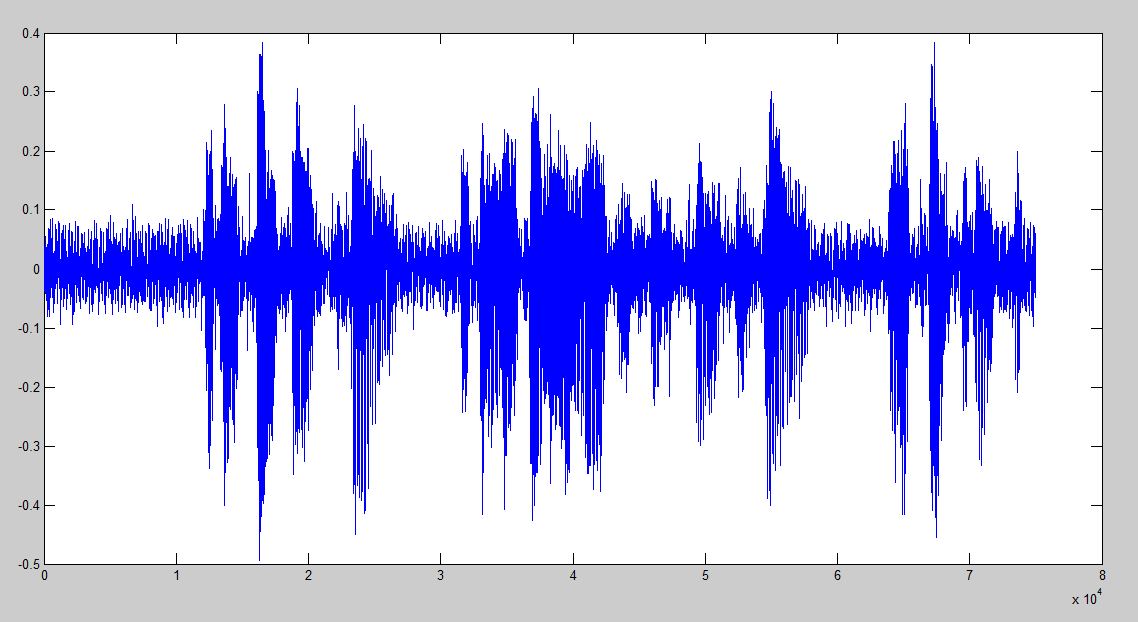
\includegraphics[width=60mm]{noisytime}}
\subfigure[After processing]{\label{fig:cleantime}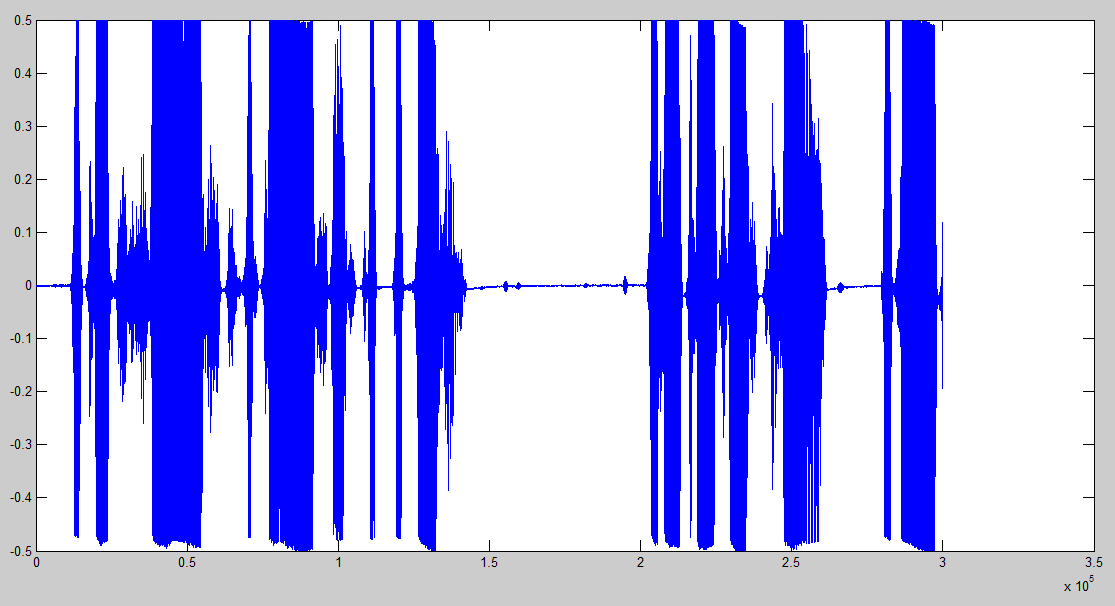
\includegraphics[width=60mm]{cleantime}}
\caption{Time domain comparison of our algorithm}
\label{fig:timecomparison}
\end{figure}

\begin{figure}
\centering     %%% not \center
\subfigure[Before processing]{\label{fig:noisyfreq}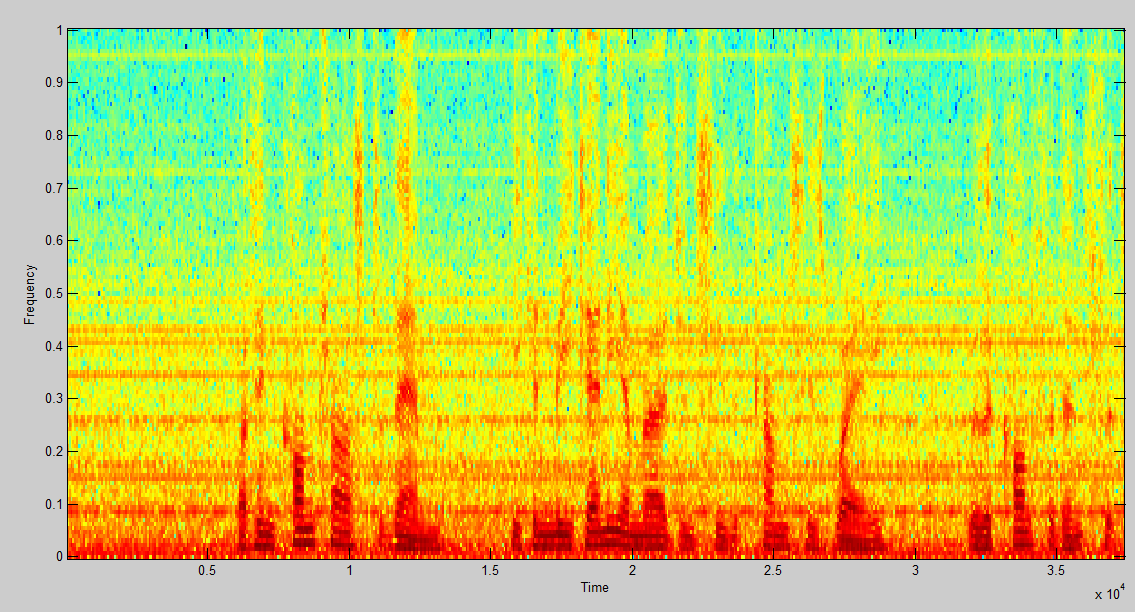
\includegraphics[width=60mm]{noisyfreq}}
\subfigure[After processing]{\label{fig:cleanfreq}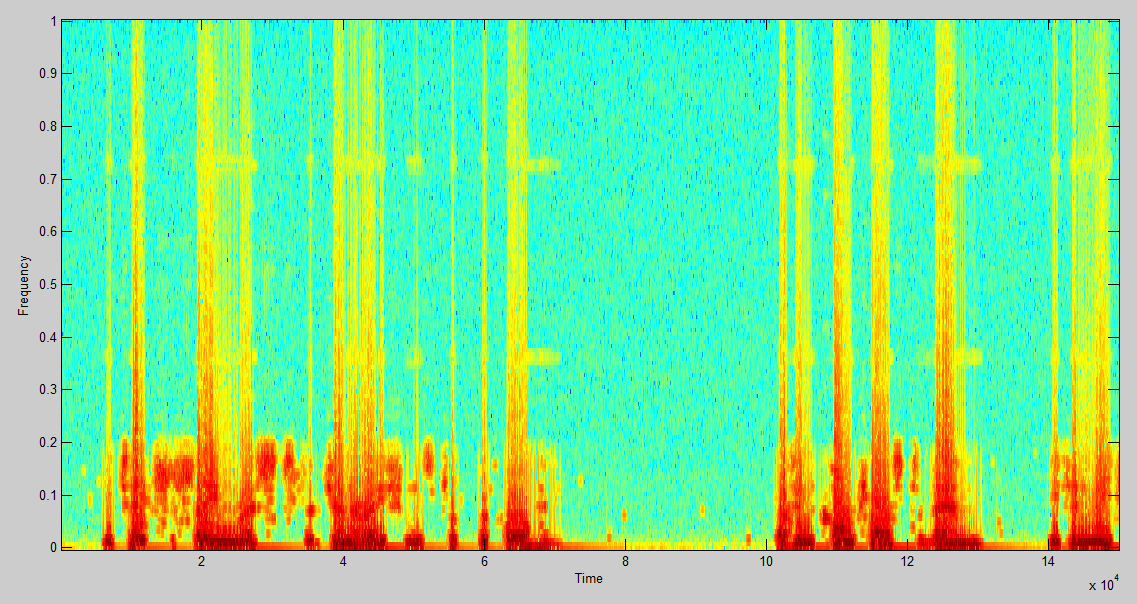
\includegraphics[width=60mm]{cleanfreq}}
\caption{Frequency domain comparison of our algorithm}
\label{fig:freqcomparison}
\end{figure}






\section{Potential Future Improvements} 

Due to time being limited we could not implement everything that we would like. Though we include here some brief discussions of enhancements that we could have implemented. 

\subsection{Longer Look Ahead Musical Noise Reduction}
Section~\ref{sec:musicalNoise} describes the technique of removing isolated high SNR frames from the output surrounded by low SNR frames, as they are unlikely to contain speech. This technique seemingly would benefit from being extended to a larger look ahead period. Rather than just having 3 frames considered (current, future and past), lasting a total of 90ms, we would look ahead around 200ms.
If we assume the minimum length of a useful utterance is around 150-200ms then we could have enough information to distinguish between musical noise and short utterances. For test cases such as the factory environment, this kind of lookahead could help us eliminate the percussive sounds in the background. 

The main downsides of this technique are increased memory requirements and an increase in the latency of the system. Increased memory usage is due to the need for an extended buffer to hold the lookahead data; the increased latency arises due to us having to be processing data with future input data in hand, therefore the latency increases by the amount of look ahead time we require. 

\subsection{Voice profiling}
Due to the nature of the samples all containing the same signal, we could profile all of the frequencies that are (significantly) present, then used multiple bandpass filters to allow only these bands through for continued processing. One could suggest that this would not be in the spirit of real time signal extraction, because we would be filtering the input data based of pre-prepared knowledge of the signal. In fact the demonstration paragraph that forms the signal is designed specifically to represent the majority of vocal patterns that are present in normal speech, and as such a frequency spectrum of the signal is representative of all speech. Naturally this filter will be more effective with a medium toned male voice than any other, but could be generalised by taking the union of a number of representative voice samples. 

A filter such as this would remove very high and very low frequencies before any of the other techniques are applied, as the human voice has the majority of its energy in the 300Hz to 1kHz region, though it would not exclude small portions in the higher register responsible for "s" and "t" sounds, thus making the output more intelligible than using just a simple band pass filter.

\section{Conclusion}

This project has exercised some interesting techniques to perform noise removal using spectral subtraction. Several improvements to the naive method have been implemented. These include various ways of tracking the noise and signal powers and shaping the output filter accordingly. Further, we have developed a feature which will completely remove components with insufficient SNR, rendering a completely clean signals when the input SNR is sufficient. In addition, we have implemented a heuristic which takes into consideration the temporal characteristics of speech, in an attempt to eliminate short bursts of noise. Finally, we discuss some improvements to the aforementioned heuristic, and discuss the potential use of voice profiling.

\clearpage

\section{APPENDIX}
\renewcommand{\thesubsection}{\Alph{subsection}}
\subsection{Simple Implementation} 
\label{app:simple}

This is the standard implementation as described in Section~\ref{sec:simple}. No special modifications have been made. 
  \begin{center}
    \begin{lstlisting}[language = C]
fft(FFTLEN, procframe);
									
static int MRotate_ctr = 0;

if (MRotate_ctr == MrotateFramecount){

	MRotate_ctr = 0;

	//rotate Mbuffs
	float* rottemp = Mbuffs[NumMbuff-1];
	for (i = NumMbuff-1; i != 0; --i)
		Mbuffs[i] = Mbuffs[i-1];
	Mbuffs[0] = rottemp;

	//Init new mbuff
	clearM = 1;
} else {
	MRotate_ctr++;
	clearM = 0;
}

for (k = 0; k < FFTLEN; ++k)
{
	float curramp = cabs(procframe[k]); 
	float currnoisebin = Mbuffs[0][k] = clearM ? curramp : min(Mbuffs[0][k], curramp);
	for (i = 1; i < NumMbuff; ++i)
		currnoisebin = min(currnoisebin, Mbuffs[i][k]);

	currnoisebin *= alpha;

	float g = max(lambda, 1-(currnoisebin/curramp));
	procframe[k] = rmul(g, procframe[k]);
}

ifft(FFTLEN, procframe);

    \end{lstlisting}
  \end{center}

\clearpage

 \subsection{Implementation using Low Pass Filtered minimum amplitude} % (fold)
 \label{sub:implementation_using_low_pass_filtered_minimum_amplitude}
 \begin{center}
 	\begin{lstlisting}[language = C]
fft(FFTLEN, procframe);
									
static int MRotate_ctr = 0;

if (MRotate_ctr == MrotateFramecount){

	MRotate_ctr = 0;

	//rotate Mbuffs
	float* rottemp = Mbuffs[NumMbuff-1];
	for (i = NumMbuff-1; i != 0; --i)
		Mbuffs[i] = Mbuffs[i-1];
	Mbuffs[0] = rottemp;

	//Init new mbuff
	clearM = 1;
} else {
	MRotate_ctr++;
	clearM = 0;
}

for (k = 0; k < FFTLEN; ++k)
{
	float curramp = cabs(procframe[k]); 

	//LPF curramp
	curramp = (1-kop1)*curramp + kop1*ampbinstate[k];
	ampbinstate[k] = curramp;

	float currnoisebin = clearM ? curramp : min(Mbuffs[0][k], curramp);
	Mbuffs[0][k] = currnoisebin;

	for (i = 1; i < NumMbuff; ++i)
		currnoisebin = min(currnoisebin, Mbuffs[i][k]);

	currnoisebin *= alpha;

	float g = max(lambda, 1-(currnoisebin/curramp));
	procframe[k] = rmul(g, procframe[k]);
}

ifft(FFTLEN, procframe);
 	\end{lstlisting}
 \end{center}

\clearpage

  \subsection{Look Ahead, Low Pass Filtered Power} % (fold)
 \label{app:delayprepipe}
 \begin{center}
 	\begin{lstlisting}[language = C]
	for (k = 0; k < FFTLEN; ++k)
	{
		float curramp = cabs(procframe[k]);
		float currpow = curramp * curramp;

		//LPF currpow
		currpow = (1-kop1)*currpow + kop1*powbinstate[k];
		powbinstate[k] = currpow;

		float currnoisebin = clearM ? currpow : min(Mbuffs[0][k], currpow);
		Mbuffs[0][k] = currnoisebin;

		for (i = 1; i < NumMbuff; ++i)
			currnoisebin = min(currnoisebin, Mbuffs[i][k]);

		currnoisebin *= alpha;
		
		lastallbinpower += currnoisebin;
		
		float powratio = currnoisebin/currpow;//(curramp*curramp);
		float g = (powratio > (nonlinclip * (allbinpower/**allbinpower*/))) ? 0 : max(lambda, 1-sqrt(powratio));
		procframeprepipe[k] = rmul(g, procframeprepipe[k]);
	}

	complex* tempframe = procframeprepipe;
	procframeprepipe = procframe;
 	procframe = tempframe;
	
	ifft(FFTLEN, procframe);
 	\end{lstlisting}
 \end{center}
 % subsection implementation_using_low_pass_filtered_minimum_amplitude (end)

% \subsection{Notes} % (fold)
% \label{sec:notes}
% \begin{itemize}
% 	\item We tried matlab, and we did slightly better (in our opinion, elaborate!)
% 	\item Try to find some sort of research paper based method, becase of research paperness
% 	\item Nonlinear clipping: inspiration = skype: see if skype has some papers on it?
% 	\item Do voice vs not voice spectral regions/singature and shape a filter for voice frequencies.
% 	\item If time > something large: do eigenvoices (perhaps talk about them anyway)
% 	\item Matlab up some figs of "hey look it is quit when he is not speaking"

% \end{itemize}
% % section notes (end)

\end{document}